\documentclass{article}

% Latex Tutorial beginners: http://www.latex-tutorial.com/tutorials/beginners/
\newcommand{\comment}[1]{}

\newcommand{\seq}[0]{$P_{seq}$}
\newcommand{\man}[0]{$P_{man}$}
\newcommand{\ndpn}[0]{$P_{nest}$}
\newcommand{\ndpv}[0]{$P_{vect}$}

\newcommand{\note}[1]{{\tiny (#1)}}

\newcommand{\algo}[0]{Histogram Balancing}

\newcommand{\gmax}[0]{\textrm{gmax}}

\newcommand{\range}[2]{$[#1,...,#2]$}

% Packages explained - Adding more functions to LATEX http://www.latex-tutorial.com/tutorials/beginners/lesson-3/
\usepackage[utf8]{inputenc}     % Zum verwenden von ä,ü und ö: http://en.wikibooks.org/wiki/LaTeX/Special_Characters
\usepackage{booktabs}
\usepackage{url}
\usepackage{hyperref}
\usepackage[T1]{fontenc}
\usepackage[normalem]{ulem}
\usepackage[margin=1.3in]{geometry}
\usepackage{graphicx}
\usepackage{amsmath}
\usepackage{listings}

\lstset{
  frame=none,
  xleftmargin=2pt,
  belowcaptionskip=\bigskipamount,
  captionpos=b,
  escapeinside={*'}{'*},
  language=haskell,
  tabsize=2,
  gobble=6,
  emphstyle={\bf},
  commentstyle=\it,
  stringstyle=\mdseries\rmfamily,
  showspaces=false,
  keywordstyle=\bfseries\rmfamily,
  columns=flexible,
  basicstyle=\small\sffamily,
  showstringspaces=false,
  morecomment=[l]\%,
}

% Erzeugen des PDF (ohne References):
% Strg + Alt + 1 in Gedit

% Erzeugen des PDF (mit References):
% Strg + Alt + 1 in Gedit
% $ bibtex expose
% Zweimal: Strg + Alt + 1 in Gedit

% fügt die Literatur auch zum Inhaltsverzeichnis hinzu (ist so nicht default)
\usepackage[notlot,notlof,numbib]{tocbibind}

% Adding a bibliography http://www.latex-tutorial.com/tutorials/beginners/lesson-7/
\bibliographystyle{apalike}


% Nested numbered enumerations, eg. 1.1, 1.2: http://tex.stackexchange.com/questions/78842/nested-enumeration-numbering
\renewcommand{\labelenumii}{\theenumii}
\renewcommand{\theenumii}{\theenumi.\arabic{enumii}.}


\title{
    Progress Report 2 \\[7pt]
    \large Nested Data Parallelism for\\ Image Processing Algorithms
}
\date{25.05.2015}
\author{Chandrakant Swaneet Kumar Sahoo}

\begin{document}

  \pagenumbering{arabic}
  
  \maketitle
  
  \paragraph{Summary}
    This is the second progress report on my thesis. After giving a summary of my
    work and my fuutre plans, I show my remaining tasks and give a
    impression of the algorithms and the code transformation.
  
  \newpage
  
  \tableofcontents
  
  \newpage
  
  \section{Leading question}
  Given a slightly irregular algorithm like \algo.
  \paragraph{How can we implement this high-level irregularly-parallel algorithm such that it compiles to efficient mashine level code?}
  \paragraph{Subquestions}
      \begin{itemize}
      \item \sout{How much faster} \emph{How easy to code and efficient in runtime} is a parallel variant against the sequential one?
      \item \sout{How much faster} \emph{How easy to code and efficient in runtime} is a compiled variant to human-written low-level parallel code?
      \end{itemize}
  
  \paragraph{Programs}
    The following name for the source codes are given. These programs are already written/transformed.
    
    \subparagraph{\seq}
       A sequential implementation using arrays of pointers and maps written in < 30min.
        
    \subparagraph{\man}
        An advanced implementation which tries to focus on efficiency.
        it uses simple top-level parallization and bytearrays to achive this.
        also written in < 30min.
        
     \subparagraph{\ndpn}
        An advanced implementation which can parallelize on every level.
        Form the view of the programer, it seems to use nested pointer-based arrays
        called \texttt{[:a:]}. They are very inefficient if implemented directly
        - however, \ndpn is automatically transformed to \ndpv and optimised by the compiler before its executed.
        also written in < 30min.
        
     \subparagraph{\ndpv}
        The highly optimized program generated by the compiler.
        It uses an type-dependent pointer-avoiding flat representation
        of the user array. I needed > 30 hours to make this transformation.
        And there is still more space to optimise.
      
  \section{Previous work}
    I have implemented all three forms of the algorithm and have almost
    finished transformations and optimizations done by the compiler.
    The optimizations by the compiler is an almost never-ending task,
    as the compiler can produce so much code, such that it were
    a few meters high if printed on paper.
    
    Initially, I was considering to show the benefits in a scalar and
    lifted call of the histogram balancing function. The function
    \texttt{hbalanceBulk} in the \ndpn-implementation - which looks exactly like
    the other implementations - is actually more expressive than it looks like.
    I had planned to show the transformed version of this code to show which optimizations it can achieve.
    However, the program transformation is quite tiresome (see. Section "Code Transformation") and
    I abandoned this idea after a week(\note{it would double-my already stuffed work...}). However, I think that this is an important aspect.
    
    I have also started analysing the algorithms and did some early (inaccurate) analysis.
    They can be found in the accompanied document \note{cost-centre.pdf}
    
    Please give me feedback on the algorithms, my current progress and especially on further analysis of \texttt{hbalanceBulk}!!
    I can still give some basic analysis of the bulk-application case, even though I won't manually
    finish its transformation.
    
  \section{Future work}
    As my next important step. I will make an more accurate program analysis- for that I will
    also finish the last optimizations I can do on the transformed program.
    
    And after that:
    I will write down all my work until the current point, maybe including the general introduction.
    It will allow me to retrace any mistakes I have done yet. This task will also significantly benefit the quality of my thesis text,
    since I can now also focus on collecting all of any tiny bits.
    I have already written a bit in this progress report and the accompanying cost centre document.
    
  \section{Progress}
    \begin{itemize}
      \item[80\%] Read more papers on Nested Data Parallel Haskell
      \item[60\%] Read more papers on Analysis of Parallel Progrmas
      \item[100\%] Decide on an algorithm (Histogram Balancing)
      \item[90\%] Program Transformation:
        \begin{itemize}
          \item[100\%] Desugar
          \item[100\%] Vectorization
          \item[70\%] Inlining \& Fusioning \note{means Optimization}
        \end{itemize}
      \item[100\%] Implement sequential variant
      \item[100\%] Implement manually-parallelized variant
      \item[100\%] Fix wrong implementation and redo steps of Desugaring and Vectorization
      \item[70\%] Analyse costs of direct interpretation of \ndpn \note{needs more accuracy}
      \item[0\%] Analyse and discuss runtime costs of vectorized interpretation of \ndpn
      \item[0\%] Analyse and discuss runtime costs of sequential implementation
      \item[0\%] Analyse and discuss runtime costs of vector-parallel implementation
      \item[0\%] Analyse and discuss human workload for the implementations
      \item[0\%] Show differences between NDP and vector-parallel
      \item[0\%] Answer first subquestion
      \item[0\%] Answer second subquestion
      \item[?\%] \textit{stuff}
      \item[0\%] Writte thesis
      \item[0\%] Colloquium
    \end{itemize}
    
  \newpage
    
  \section{Time Table}
    \begin{table}[h]
      \begin{center}
      \caption{Time table} % http://www.latex-tutorial.com/tutorials/beginners/lesson-8/
      \label{timetable}
      \begin{tabular}{lrrl}
        \toprule
        Current Week & CW & monday & thesis work \\
        \midrule
            & 17 & 20.04 & reading remaining papers, reading parallel complexity theory \\
            & 18 & 27.04 & deciding on an algorithm  \\
            & 19 & 4.05  & implementing \ndpn, vectorizing and optimizing \ndpn \\
            & 20 & 11.05 & implementing \seq and \man, vectorizing and optimizing \ndpn \\
            & 21 & 18.05 & vectorizing and optimizing, rereading details of implementation, analysis \\
        now & 22 & 25.05 & finish transformation, analysis \& comparision\\
            & 23 & 1.06  & \sout{\textit{puffer}} analysis \& comparision \\
            & 24 & 8.06  & \textit{puffer} \\
            & 25 & 15.06 & Begin to write down, prepare for exams\\
            & 26 & 22.06 & Writing..., prepare for exams \\
            & 27 & 29.06 & Writing..., prepare for exams \\
            & 28 & 6.07  & Prepare Colloquium, Writing..., exams week 1 \\
            & 29 & 13.07 & Prepare Colloquium, Finalize writing, exams week 2 \\
            & 30 & 20.07 & Colloquium and Release \\
            & 31 & 27.07 & Last week for Colloquium and Release \\
            & 32 & 3.08  & Fin \texttt{:D} \\
      \end{tabular}
      \end{center}
    \end{table}
  
  \section{Recommended Literature}
  
    I have come over the following papers.
    The papers are sorted by their relevance.
    The percentage shows how much of each paper I have throughly read.
    You are recommended to read the essential papers. Important ones
    are included in \textrm{Papers.zip}.
    
    \paragraph{Essential}
      \begin{itemize}
        \item[100\%] Data Parallel Haskell: A Status Report \cite{DPHStatus2007}
        \item[100\%] Harnessing the Multicores: Nested Data Parallelism in Haskell \cite{Harness2008}
        \item[100\%] Data Parallel Haskell - 2010 Video - {S.P}. Jones \cite{Simon2010Video}
        \item[100\%] Programming Parallel Algorithms \cite{Blelloch:1996:PPA:227234.227246}
        \item[100\%] On the distributed implementation of aggregate data structures by program transformation \cite{DistTypes1999}
        \item[60\%] Costing Nested Arrays Codes \cite{CostArray2002Leshchinskiy}
      \end{itemize}
      
    \paragraph{Compulsatory}
      \begin{itemize}
        \item[20\%] Higher Order Flattening \cite{HighOrdFlat2006}
        \item[100\%] Stream Fusion: From Lists to Streams to Nothing at All \cite{Fusion2007}
        \item[20\%] Exploiting Vector Instructions with Generalized Stream Fusion \cite{GenVectorFusion2013}
        \item[234324\%] JSKDFLSDF
        \item[20\%] Reevaluating Amdahl's Law \cite{Gustafson1988}
        \item[20\%] Work Efficient Higher-order Vectorisation \cite{EffiVect2012Lipp}
        \item[20\%] Playing by the Rules: Rewriting as a practical optimization technique in GHC \cite{Simon2001Rewrites}
        \item[100\%] An Approach to Fast Arrays in Haskell \cite{FastArr2003Chakravarty}
        \item[40\%] Functional Array Fusion \cite{ArrayFusion2001Chakravarty}
      \end{itemize}
      
    \paragraph{Details}
      \begin{itemize}
        \item[40\%] Systematic Efficient Parallelization of Scan and Other List Homomorphisms \cite{ParScan1996Gorlatch}
        \item[30\%] Simon Peyton Jones - Data Parallel Haskell papers \cite{Simon2013DPHpapers}
        \item[0\%] Implementation of a Portable Nested Data-parallel Language \cite{NepaBelloch1993}
        \item[60\%] More Types for Nested Data Parallel Programming (PA implementations replPA,indexPA...) \cite{TypesNested2000}
        \item[20\%] Paritial Vectorization of Haskell programs \cite{Chakravarty2008Partial}
        \item[30\%] Associated Type with Class \cite{DataFamily2005Chakravarty}
      \end{itemize}
      
    \paragraph{Alternate Approaches}
      \begin{itemize}
        \item[10\%] Composable Memory Transactions \cite{Harris2005Composable}
        \item[30\%] Algorithm + Strategy = Parallelism \cite{Trinder1998Algorithm}
        \item[20\%] Regular, Shape-polymorphic, Parallel Arrays in Haskell \cite{Keller2010Regular}
        \item[20\%] Parallel and Concurrent Programming in Haskell \cite{Marlow2012Parallel}
        \item[20\%] A monad for deterministic parallelism \cite{Marlow2011Monad}
        \item[10\%] Optimising Purely Functional {GPU} Programs \cite{McDonell2013Optimising}
      \end{itemize}
    
  \newpage
  
  \section{Algorithms}
    
    The following sections will explain the conceptiual algorithm
    and then show the the code for the \seq, \man and \ndpn implementations
    and a pseudo-interface all of them implement.
    
    \subsection{Histogram Balancing}
      Suppose we have an $w \times h$-8-bit-gray-tone image with low contrast.
      
      \begin{figure}[h]
        \centering
        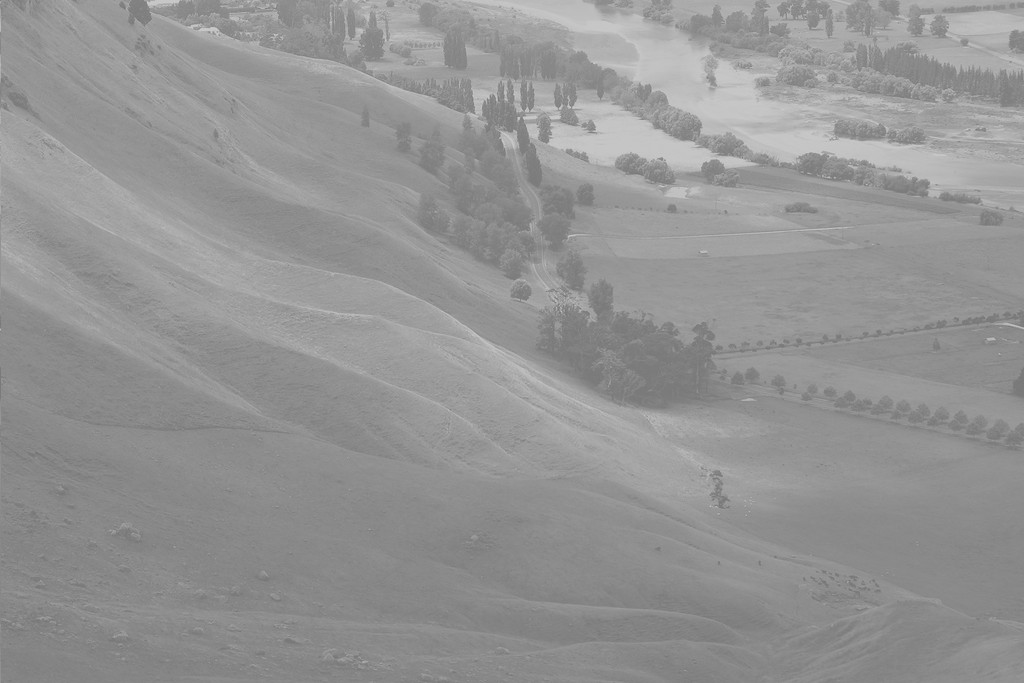
\includegraphics[width=0.45\textwidth]{img-org}
        \caption{An image with low constrast
        \footnote{photo by Phillip Capper. Source: \url{https://en.wikipedia.org/wiki/File:Unequalized_Hawkes_Bay_NZ.jpg}}
        }
        \label{fig:img-org}
      \end{figure}
      Our goal is to make details more visible to the viewer. For that,
      lets take a look at the histogram of the image.
      
      \begin{figure}[h]
        \centering
        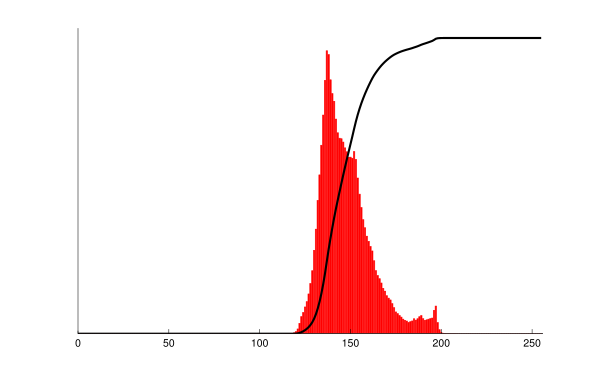
\includegraphics[width=0.45\textwidth]{hist-org}
        \caption{The histogram of the original image with absolute(red) and accumulative(black) count.
        \footnote{made by used Wikipedia user \c{Jarekt}. Source: \url{https://en.wikipedia.org/wiki/File:Unequalized_Histogram.svg}}
        }
        \label{fig:hist-org}
      \end{figure}
      
      A histogram shows the gray tone distribution of the image in interest.
      The x-axis denotes the gray tone and the y-axis denotes the
      number of pixels with a gray tone $x$ (red). The black curve denotes the
      total number of pixels with a gray tone $g \leq x$.

      We can now see, why details are difficult to recognize in our original image.
      The gray tones are tightly packed together and the
      entire image only uses values in the range \range{120}{205}.
      Histogram Balancing solves this problem by defining a mapping
      $f: Graytone \rightarrow Graytone$, such that the accumulating count
      of the resulting image increases as uniformly as possible from 0 to 255.
      The histogram \ref{fig:hist-eq} shows our goal.
      
      \begin{figure}[h]
        \centering
        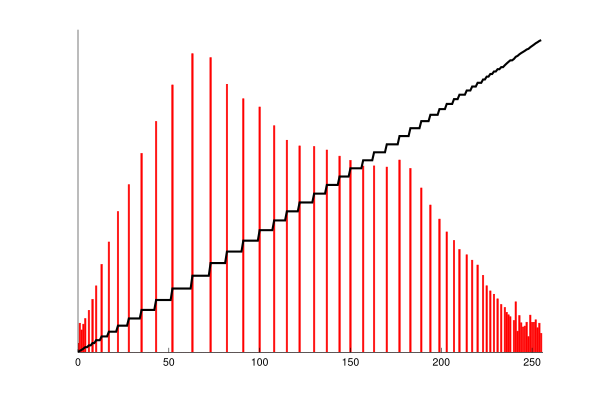
\includegraphics[width=0.45\textwidth]{hist-eq}
        \caption{The histogram of the balanced image
        \footnote{made by used Wikipedia user \c{Jarekt}. Source: \url{https://en.wikipedia.org/wiki/File:Equalized_Histogram.svg}}
        }
        \label{fig:hist-eq}
      \end{figure}
      
      Notice the new curve for the accumulating count(black). We can define
      this mapping by spreading out the gray tones such that more
      important gray tones get a larger range to occupy. We interpret
      a high histogram-value for a gray tone as a high importance.
      Given this interpretation, we can - visually - build the histogram(1),
      lay down the bars consecutively - remembering which
      bar belongs to which gray tone(2), normalize(3) and scale(4) the bars to \range{0}{255} - 
      and finally - assign each bar (and therefore its gray tone) a new gray tone
      using the bars location in the range \range{0}{255}(5). \note{I should include visual diagrams for this in the thesis.}
      
      \paragraph{}
      To define the transformation $ hbalance: Image \rightarrow Image$ we need the following definitions:
      \begin{itemize}
        \item $Image := (Width,Height,Width \times Height \rightarrow Graytone)$:
          An image
        \item $Histogram_a: Graytone \rightarrow a$:
          A histogram assigns a count to each gray tone(for $a=Int$).
        \item $\gmax: Graytone$:
          The maximum gray tone for the data type in use. (e.g. 255 for 8-bit gray tones)
        \item $hist: Image \rightarrow Histogram_{Int}$
          calculates the histogram of an image. (1)
        \item $accu: Histogram_{Int} \rightarrow Histogram_{Int}$
          calculates the accumulating histogram from the original histogram. (2)
        \item $normalize: Int \times Int \times Histogram_{Int} \rightarrow Histogram_{Double}$
          normalizes the bars (in the range defined by the first two arguments) to a range from 0 to 1. (3)
          The second argument (called $agmax$) denotes the number of total pixels in the image.
          It can be calculated with $a(\gmax)$ or $a(g)$ where $g$ is highest gray tone in the image.
          Both are equal, so the implementations take the liberty to use any of these formulas.
        \item $scale: Graytone \times Histogram_{Double} \rightarrow Histogram_{Int}$
          scales the normalized values to the maximum gray tone(255 in our case) and rounds down to the nearest integer. (4)
        \item $apply: Histogram_{Int} \times Image \rightarrow Image$
          maps each gray tone to its new value as dictated by the first argument. (5)
      \end{itemize}
      
      Given these functions we can define $hbalance: Image \rightarrow Image$ as:
      \begin{equation}
      \begin{split}
        hbalance(img) & := apply(s,img) \\
          s & := scale(\gmax,n) \\
          n & := normalize(a(0), a(\gmax), a) \\
          a & := accu(h) \\
          h & := hist(img) \\
      \end{split}
      \end{equation}
      
      Concrete implementations are given in the next sections.
      Applying the algorithm to our initial image gives \ref{fig:img-eq}. Details are more distinguishable in our new image.
      
      \begin{figure}[h]
        \centering
        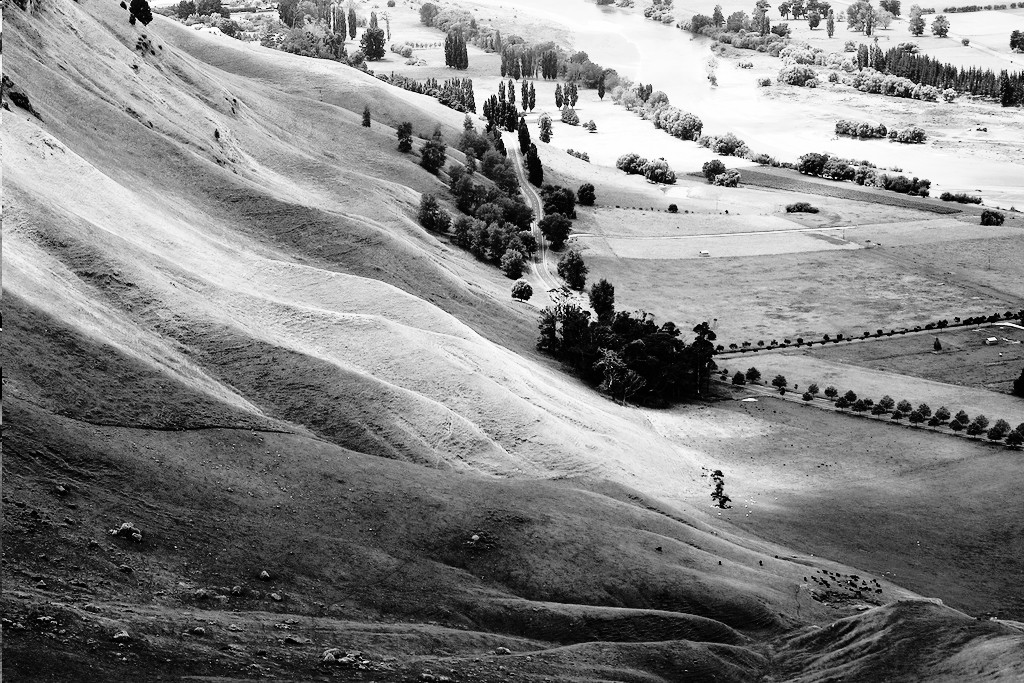
\includegraphics[width=0.45\textwidth]{img-eq}
        \caption{The equalized image
        \footnote{photo by Phillip Capper. Source: \url{https://en.wikipedia.org/wiki/File:Equalized_Hawkes_Bay_NZ.jpg}}
        }
        \label{fig:img-eq}
      \end{figure}
      
    \subsection{Pseudo-Interface}
      All implementations have to give concrete definitions for this pseudo-interface.
      It defines names for the functions and data types, so that each implementation
      can take the libery to define a different representation of images, histograms etc...
      The implementations are flexible in that the gray tone type (32-bit Int, 8-bit Int etc...)
      can be changed at any time. This is why Image takes a type parameter and why we have to
      let the program know the maximum gray tone gmax. I am calling this a pseudo-interface,
      because it resembles interfaces from Java and associated type synonyms in Haskell.
      \begin{lstlisting}
        type Image a -- the type for Images of gray-tone type a
        type Many a  -- thy type to represent bulks of images

        img :: Image Int -- this shall be an example image
        images :: Many (Image Int) -- this shall be an example collection of images
        
        hbalance :: Image Int -> Image Int -- single application of histogram balancing
        hbalanceBulk :: Many (Image Int) -> Many (Image Int) -- bulk application of histogram balancing
      \end{lstlisting}
      
      The maximum gray tone gmax in the implementations will be set to 255 although
      a much larger value is possible.
    
    \newpage
    
    \subsection{Implementation of \seq}
      This section gives the implementation of \seq and notes on it.
      \seq is a very direct implementation without strong focus on efficiency and
      was written within 30 minutes.
      
      \lstinputlisting{seq.hs}
      
      The implementation uses Haskell Vectors \footnote[1]{See vector package on Hackage: \url{http://hackage.haskell.org/package/vector-0.10.0.1/docs/Data-Vector.html}}.
      Vectors are immutable pointwise-lazy arrays and
      exhibit different behaviour than conventional C arrays.
      Immutable means, that (like every value in Haskell) their value cannot be changed after creation.
      Pointwise-lazyness basically means, that every value inside the array is not caluclated
      until its value is actually demanded. We don't need to know more than that.
      However, this means that vectors are roughly like immutable C-arrays of pointers
      where each pointer refers to the actual data on the heap.
      The implementation uses two-dimensional vectors to represent an image.
      
      Vectors can hold data of arbitrary complexity. This includes an image itself.
      Therefore we can also use a vector to represent a collection of images.
      
      The main algorithm (hbalance) is implemented pretty much like the definition.
      The representation of an histogram uses a Map data structure \footnote[2]{See containers package on Hackage: \url{http://hackage.haskell.org/package/containers-0.5.6.1/docs/Data-Map-Strict.html}}.
      A histogram is defined as a map from finitely many integer values to some fixed type a.
      The expressions for $a(0)$ and $a(gmax)$ extract the value for the smallest
      and largest gray tone from the map respectively.
      
      The other functions are now briefly explained:
      \begin{itemize}
        \item hist: The histogram calculation flattens the image to a one-dimensional vector and 
          iterates through all elements creating a map of graytones and their number of occurrences.
        \item accu: calculates the prefixsum of the gray tones counts in the map.
          The map is traversed from smaller gray tones to larger ones.
        \item normalize: fromIntegral is the explicit conversion from Double to Int.
        \item scale: Scales each value from 0 to 1 to 0 to gmax and rounds down the floating point results.
        \item apply: maps each pixel in each row by looking up (this is what M.! does) that pixels gray tone in the final equalized histogram.
      \end{itemize}
      
    \newpage
    \subsection{Implementation of \man}
      The manually-parallelized program focuses a bit more on parallelizing
      the task. Given the time constraint of 30 minutes, it can only implement
      simple optimizations for parallel behaviour. Let's take a look at its code.      
      
      \lstinputlisting{man.hs}
      
      In constrast to \seq, the two-dimensional vectors have been
      flatten into a single dimension. Images are now represented
      by a single flat unboxed vector. Such unboxed vectors use no pointers,
      are bulk-strict in their elements and are immutable as well.
      
      To retrieve a specific pixel one needs to calculate
      the offset using the images width. Fortunately,
      for histogram balancing, we don't need to retrieve pixels by their indices anyways.
      (However, other algorithms operating on these images would have to cope with that complication.)
      The unboxed vectors are stored as a contiguousblock of memory with
      the actual raw data types as values. They are the closest equvalent of classic C-arrays.
      
      Avoiding pointers and an extra level of nesting on the images 
      makes \man more efficient than the \seq - in cost of a more complicated implementation.
      Also note that, unlike normal (boxed) vectors,
      unboxed vectors cannot contain every data type.
      (Because, if you want to avoid pointers, you need to know the size of the
      elements in advance to allocate the space for it. This is not possible for complex
      types like lists, trees or even vectors.)
      This is the reason, why a colleciton of images is represented by a
      (boxed) vector (just like in \seq).
      
      However, the efficient representation of images comes at a (possibly high) cost.
      Since unboxed vectors are bulk-strict and immutable,
      its not possible to parallelize the construction/calculation of it's elements.
      That would either require mutability and explicit spawning and synchronization of threads,
      or a fallback to boxed vectors.
      The first option greatly increases the complexity of the program
      and the time to implement it. Though possible in Haskell, I choose
      against it, to keep my implementation understandable, simple and bug-free.
      The second option is viable, since boxed vectors allow for parallel
      evaluation very easily. However, as mentioned, they use pointers and introduce great constant factor slowdown during execution.
      Therefore hbalance itself is essentially implemented sequentially.
      (An Prof. Bußmeier: \textasciicircum Bitte unbedingt diskutieren, inwiefern ich stattdessen eine parallelisierbare aber pointer-basierte implementation nehmen soll. Der Aufwand stiege von 30min auf ca 1h. \textasciicircum )
      
      Since the collection of images itself is stored in a unboxed vector,
      it's evaluation can be parallelized. The definition of hbalanceBulk
      uses \cite{Trinder1998Algorithm} to parallelize the work.
      Operationally, the expression spawns cores-many threads, assigns
      each thread a chunk of the entire collection of images,
      makes each thread process it's chuck sequentially, and finally joins the threads.
      (More presicely, it evaluates the elements to (Weak Head) Normal Form in parallel
      instead of evaluating them sequentially as usual.)
      
      The remaining functions are implemented very much like in \seq.
      The only main difference is the representation of the histogram as an unboxed vector instead of a Map.
      An unboxed vector of length $\gmax+1$ is used where the element at
      index $i$ denotes the number of pixels with gray tone $i$,
      e.g. a vector $ [0,3,4] $ represents the histogram $ \{0 \mapsto 0, 1 \mapsto 3, 2 \mapsto 4 \}$.
      
    \newpage
    
    \subsection{Implementation of \ndpn}
      We can now finally discuss the main implementation of my thesis. This
      implementation uses Nested Data Parallelism \cite{Harness2008} and
      is the most promising one from all three implemetations.
      It was written in < 30 minutes and was easier to write than \man.
      in code, \lstinline|[:a:]| refers to a parallel array of type a. The various common
      functions over lists (map,group,sort,etc.) have been replicated for arrays and have a P suffix appended (e.g. mapP).

      \lstinputlisting{ndpn.hs}
      
      The implementation uses polymorphic type-indexed bulk-strict arrays \lstinline|[:a:]|
      to represent an image and a collection of images.
      Contrary to it's appearance, parallel arrays of this type are more
      flexible than vectors and on average comparably efficient. I won't
      repeat it's features and semantics now and refer to \cite{Harness2008}.
      
      Except for hist, the entire implementation is very similar to the original definition
      and to \man. However, in this case the entire implementation
      of hbalance is also parallel - and even distributed!
      
      The definition of hist uses an alternative way to build the histogram.
      This is where previous implementation used an iteration
      over all values to compute the histogram. This implementation instead
      uses bulk-operations to group together the gray tones and count them in parallel.
      This implementation, to me personally, looks more elegant than the iterative
      implementation in \seq and \man. To our benefit, it is also more parallelizable
      than the others.
  
  \newpage
  
  \section{Code Transformation}
    This section briefly shows the code resulting from applying
    the transformations described in \cite{Harness2008} on \ndpn.
    The transformations are not commented yet and not entirely finished.
    (Stream and communication fusion at the end is still missing.)
    I needed much time to make these transformations - as they are ususally
    the compilers work. You can see the full, step-by-step, transformations on my github repository \footnote[1]{In the top-level files at \url{https://github.com/GollyTicker/Nested-Data-Parallel-Haskell/tree/64abb73dcc50ee39816f8d02a18fbb00b48d7b57}}.

    After the transformations of the individual functions, the entire
    desugared and vectorized function and my current progress in on optimization is shown.
    I don't expect the code to be understood yet - therefore I don't give explanations now.
    
    I have also ommitted the lifted variants of the code.
    
    \note{I some sense, I want to show that I have not been slaking around doing nothing in 3/4 weeks.}
    
    \subsection{Individual functions in \ndpn}
    
      \subsubsection{hbalance}
        
        \lstinputlisting[xleftmargin=3em]{hbalance.hs}
        
      \subsubsection{hist}
        
        \lstinputlisting[xleftmargin=3em]{hist.hs}
        
      \subsubsection{accu}
        
        \lstinputlisting[xleftmargin=3em]{accu.hs}
        
      \subsubsection{normalize}
        
        \lstinputlisting[xleftmargin=3em]{normalize.hs}
        
      \subsubsection{scale}
        
        \lstinputlisting[xleftmargin=3em]{scale.hs}
      
    \subsection{Vectorized \ndpn }
      
      \lstinputlisting[xleftmargin=3em]{vectorized.hs}
  
    \subsection{Partially optimised \ndpn}
      
      \lstinputlisting[xleftmargin=3em]{optimised.hs}
  
  
  \newpage
  
  \bibliography{report2}
  
\end{document}

